\subsection{Httpd Script}
\begin{figure}[htp]
\centering
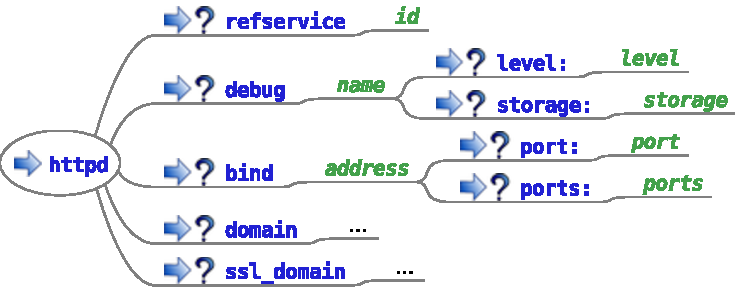
\includegraphics[width=0.64\textwidth]{httpd_service_script}
\label{fig:httpd_service_script}
\caption{Httpd Script Statements}
\end{figure}

\begin{figure}[htp]
\centering
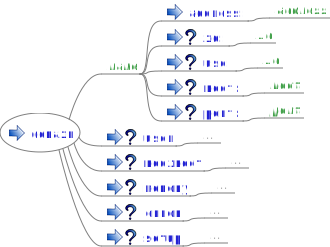
\includegraphics[width=0.5\textwidth]{httpd_domain_script}
\label{fig:httpd_domain_script}
\caption{Httpd Domain Statements}
\end{figure}

\begin{figure}[htp]
\centering
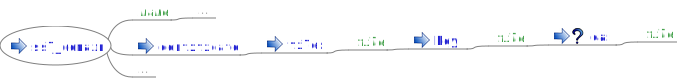
\includegraphics[width=0.99\textwidth]{httpd_ssldomain_script}
\label{fig:httpd_ssldomain_script}
\caption{Httpd SSL/Domain Statements}
\end{figure}

\begin{figure}[htp]
\centering
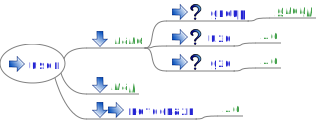
\includegraphics[width=0.45\textwidth]{httpd_user_script}
\label{fig:httpd_user_script}
\caption{Httpd Domain User Statements}
\end{figure}

\begin{figure}[htp]
\centering

\includegraphics[width=0.35\textwidth]{httpd_redirect_script}
\label{fig:httpd_redirect_script}
\caption{Httpd Redirect Statements}
\end{figure}

\begin{figure}[htp]
\centering

\includegraphics[width=0.8\textwidth]{httpd_memory_script}
\label{fig:httpd_memory_script}
\caption{Httpd Memory Statements}
\end{figure}

\begin{figure}[htp]
\centering

\includegraphics[width=0.8\textwidth]{httpd_error_script}
\label{fig:httpd_error_script}
\caption{Httpd Error Statements}
\end{figure}


%% httpd
\TheStatement{httpd}
\TheStatement*[httpd]{httpd \{ refservice bind debug domain ssl\_domain \}}

Entry point in the httpd script.

%% refservice
\TheStatement[httpd:refservice]{refservice}
\TheStatement*[httpd!refservice]{refservice \Arg{name}}

If in the used profile script there is was a service ID set,
that service ID can be references by the \Arg{name}, so that 
two or more different Httpd services on the server can be installed.
The following example will have two services with the IDs \qcode{idone}
and \qcode{idtwo} that will install the services \qcode{apache} and
\qcode{nginx}, respectively.

\begin{lstlisting}[style=Java,caption={Profile with the services IDs "UbuntuProfile.groovy".}]
profile "ubuntu_12_04", {
    httpd {
        service ["idone": "apache", "idtwo": "nginx"]
    }
}
\end{lstlisting}

\begin{lstlisting}[style=Java,caption={Script "HttpdOne.groovy"}]
httpd {
    // reference service with id "idone"
    refservice "idone"
}
\end{lstlisting}

\begin{lstlisting}[style=Java,caption={Script "HttpdTwo.groovy"}]
httpd {
    // reference service with id "idtwo"
    refservice "idtwo"
}
\end{lstlisting}

%% debug
\TheStatement[httpd:debug]{debug}
\TheStatement*[httpd!debug level]{debug \Arg{name}, level: \Arg{name}}

Sets the logging \Arg{level} for the debug category \Arg{name}. The category
is specific for the Httpd service.

\begin{lstlisting}[style=Java]
httpd {
    debug "error", level: 1
}
\end{lstlisting}

\TheStatement*[httpd!debug storage]{debug \Arg{name}, storage: \Arg{storage}}

Sets the logging \Arg{storage} for the debug category \Arg{name}. The category
is specific for the Httpd service.

\begin{lstlisting}[style=Java]
httpd {
    debug "error", storage: "/var/log/nginx/error.log"
}
\end{lstlisting}

%% bind
\TheStatement[httpd:bind]{bind}
\TheStatement*[httpd!bind]{bind local|all|\Arg{address}, port: \Arg{port}|ports: \Arg{ports}}

The IP \Arg{address} or a list of \Arg{addresses} or the host name(s) and
the \Arg{port} or list of \Arg{ports} on which the web server should listen 
to connections. Set to \qcode{local} for the local host 
address \code{127.0.0.1} or to \qcode{all} to listen to all hosts.

\begin{lstlisting}[style=Java]
httpd {
    bind local, port: 80
    bind all, port: 80
    bind "192.168.0.1", ports: [80, 443]
}
\end{lstlisting}

%% domain
\TheStatement[httpd:domain]{domain}
\TheStatement*[httpd!domain]{domain \Arg{name}, address: \Arg{address} [, id: \Arg{id}] [, use: \Arg{id}] [, root: \Arg{root}] [, port: \Arg{port}], \{ user redirect setup \}}

Creates a new domain with the \Arg{name} and the \Arg{address} on the server.
The domain can have an optional unique identifier \Arg{id} that can be 
references from other domain. The domain have the default \Arg{port} of 80 but can 
be changed to any other port, if the server will not serve the web site on the
standard HTTP port. 
Optionally, the identifier \Arg{id} of the domain which parameters 
should be used can be set with the \qcode{use} statement. 
Optionally, the domain \Arg{root} directory with the \qcode{root} 
statement can be set. 

\begin{lstlisting}[style=Java]
httpd {
    domain "test1.com", address: "192.168.0.50", {
    }
}
\end{lstlisting}

%% ssl_domain
\TheStatement[httpd:ssl_domain]{ssl_domain}
\TheStatement*[httpd!ssl\_domain]{ssl\_domain \Arg{name}, address: \Arg{address} [, id: \Arg{id}] [, use: \Arg{id}] [, root: \Arg{root}] [, port: \Arg{port}], \{ certificate user redirect setup \}}

Creates a new SSL domain with the \Arg{name} and the \Arg{address} on the server.
The domain can have an optional unique identifier \Arg{id} that can be 
references from other domain. The domain have the default \Arg{port} of 443 but can 
be changed to any other port, if the server will not serve the web site on the
standard HTTPS port. 
The certificate for the domain must be set.
Optionally, the identifier \Arg{id} of the domain which parameters 
should be used can be set with the \qcode{use} statement. 
Optionally, the domain \Arg{root} directory with the \qcode{root} 
statement can be set. 

\begin{lstlisting}[style=Java]
httpd {
    ssl_domain "test1.com", address: "192.168.0.50", {
        certificate ...
    }
}
\end{lstlisting}

%% user
\TheStatement[httpd:domain:user]{user}
\TheStatement*[httpd!domain!user name]{user \Arg{name} [, group: \Arg{name}] [, uid: \Arg{id}] [, gid: \Arg{id}]}\\
\TheStatement*[httpd!domain!user map]{user \Arg{map}}\\
\TheStatement*[httpd!domain!user refdomain]{user refdomain: \Arg{id}}\\

Sets the domain local user under which the services from this domain are 
run under. Sets the user \Arg{name} and optionally the user group \Arg{name},
the user identifier \Arg{id} and the user group identifier \Arg{id}. The
statements of the user can be set with a map where the keys correspond to the
statements. Otherwise, a different domain can be references with 
the \qcode{refdomain} statement so that the user of the referenced domain
will be used for this domain.

\begin{lstlisting}[style=Java]
domainUser = [user: "foouser", uid: 2005, group: "foogroup", gid: 2005]

httpd {
    domain "test1.com", address: "192.168.0.50", {
        // use the map "domainUser"
        user domainUser
    }
}
\end{lstlisting}

\begin{lstlisting}[style=Java]
httpd {
    domain "test1.com", id: domain1id, address: "192.168.0.50", {
    }
    ssl_domain "test1.com", address: "192.168.0.50", {
        // reference the user of the domain "domain1id"
        user refdomain: domain1id
    }
}
\end{lstlisting}

%% redirect
\TheStatement[httpd:domain:redirect]{redirect}
\TheStatement*[httpd!domain!redirect]{redirect [from: \Arg{host},] to: \Arg{host}}

Redirects requests from the \Arg{host} set in the \qcode{from} statement 
to the \Arg{host} set in the \qcode{to} statement. The from host defaults
to the current domain. The placeholder \qcode{\%} can be used for the current
domain name. If no protocol is set than it is assumed to be the same as of 
the current domain, i.e. insecure domains uses the protocol \qcode{http://}
and secure domains uses the protocol \qcode{https://}.

\begin{lstlisting}[style=Java]
httpd {
    // redirects to the www sub-domain
    domain "test1.com", id: domain1id, address: "192.168.0.50", {
        redirect to: "www.%"
    }
    // redirects to the secure connection
    domain "test2.com", id: domain1id, address: "192.168.0.50", {
        redirect to: "https://www.%"
    }
    // redirects from the path to the domain
    domain "test3.com", id: domain1id, address: "192.168.0.50", {
        redirect from: "%/some", to: "http://foo.com"
    }
}
\end{lstlisting}

%% memory
\TheStatement[httpd:domain:memory]{memory}
\TheStatement*[httpd!domain!memory]{memory limit: \Arg{size} [, upload: \Arg{size}] [, post: \Arg{size}]}

Sets the memory limit for scripts, uploads and posts. The memory \Arg{size}
can be set in units of $\mathrm{byte|kB,MB,\dots,YB|KiB,MiB,\dots,YiB}$.
If the upload and post memory limits are not set, the memory limit is used set
by the \qcode{limit} statement.

\begin{lstlisting}[style=Java]
httpd {
    // sets the script, upload and post memory limit
    domain "test1.com", address: "192.168.0.50", {
        memory limit: "32 MB"
    }
    // redirects to the secure connection
    domain "test2.com", address: "192.168.0.50", {
        memory limit: "32 MB", upload: "32 MB", post: "32 MB"
    }
}
\end{lstlisting}

%% error
\TheStatement[httpd:domain:error]{error}
\TheStatement*[httpd!domain!error page]{error page: \Arg{page}}
\TheStatement*[httpd!domain!error root]{error root: \Arg{path}}
\TheStatement*[httpd!domain!error errorCodes]{error errorCodes: \Arg{codes}}

Sets the error \Arg{page}, the root directory \Arg{path} of the pages and 
the error \Arg{codes} for which the pages are displayed.

\begin{lstlisting}[style=Java]
httpd {
    domain "test1.com", address: "192.168.0.50", {
        error page: "/50x.html"
    }
    domain "test2.com", address: "192.168.0.50", {
        error page: "/50x.html", codes: "500, 502, 503, 504", root: "/usr/share/nginx/html"
    }
}
\end{lstlisting}

%% certificate
\TheStatement[httpd:domain:certificate]{certificate}
\TheStatement*[httpd!domain!certificate]{certificate file: \Arg{file}, key: \Arg{file} [, ca: \Arg{file}]}

Sets the certificate \Arg{file}, the certificate key \Arg{file} and optionally the
certificate authority \Arg{file} for the domain.

\begin{lstlisting}[style=Java]
httpd {
    ssl_domain "test1.com", address: "192.168.0.50", {
        certificate file: "test1.com.crt", key: "test1.com.key", file: "test1-ca.com.crt"
    }
}
\end{lstlisting}

